% !TeX root = ../FinalRepordCS.tex

\chapter{Related Work}
According to the previous research, some methods of key generation based on the physical layer of the LoRa communication protocol were proposed. However, Physical layer key generation for LoRa is still under development, but it has the potential to revolutionize the security of LoRa-based networks. It can be used to secure a wide range of applications, including smart cities, industrial automation, and the Internet of Things.
Physical layer key generation for LoRa is a promising technique for establishing secure communication links in LoRa-based networks. Physical layer key generation exploits the randomness and reciprocity of the LoRa channel to extract a secret key shared by the communicating devices. This key can then be used to encrypt and decrypt their communication, ensuring confidentiality and integrity.

\section{Theoretical Foundations}

\subsection{Physical Layer Key Generation}
Physical layer key generation is the way to generate a shared secret key between wireless devices by exploiting the reciprocity of the random fading channel, in which wireless devices measure highly correlated wireless channel characteristics (e.g., channel impulse responses or received signal strengths) and use them as shared random sources to generate a shared key. In theory, in a rich multipath scattering environment, a passive attacker who is more than a half-wavelength away from the legitimate users will obtain uncorrelated channel measurements and thus cannot infer much information about the generated key. The physical layer key generation mechanisms do not require expensive computation and have the potential to achieve information-theoretic security in the sense that the secrecy of the generated key is not dependent on the hardness of a computational problem but relies on the physical laws of the wireless fading channels.[3] 
Generally, physical layer key generation applies the following five steps to generate a key: channel probing, randomness extraction, quantization, information reconciliation, and privacy amplification, illustrated in Figure 2.1.
\begin{figure}
  \centering
  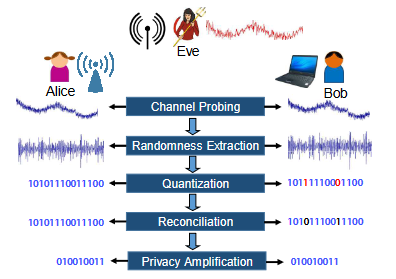
\includegraphics[width=0.6\linewidth]{fig2-1.png}
  \caption{Secret key generation model[3]}
  \label{fig:2-1}
\end{figure}

\subsection{LoRa Physical Layer Protocol}
LoRa adopts the Chirp Spread Spectrum (CSS) modulation mechanism, which provides anti-interference and long-range communication capability. As shown in Figure 2.2(a) and (b), a base symbol in LoRa physical layer protocol (PHY) is a chirp with frequency linearly increasing with time. The start frequency (fstart ) of a symbol represents the encoded information. A LoRa symbol has two segments with a sharp frequency drop, as shown in Figure 2-2(c).
\begin{figure}
  \centering
  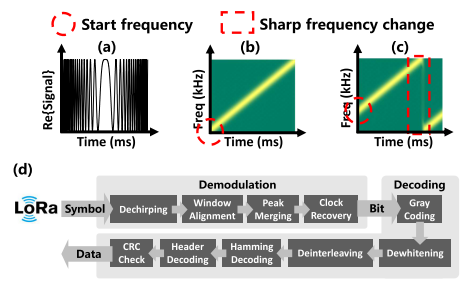
\includegraphics[width=0.7\linewidth]{fig2-2.png}
  \caption{(a) Real part of a base up-chirp symbol. (b) Base up-chirp symbol. (c) Shifted symbol. (d) Complete procedure of LoRa PHY\cite{10.1145/3546869}}
  \label{fig:2-2}
\end{figure}
And the RSSI (Received Signal Strength Indicator) is a relative measurement that helps us determine if the received signal is strong enough to get a good wireless connection from the transmitter. Since LoR supports bi-directional communication, The RSSI is an important measurement for both gateways and end devices. And RSSI is measured in dBm and its value is a negative form. The closer the RSSI value is to zero, the received signal is stronger, the good examples for positive and negative have shown in Figure 2.3 (a) and (b)\cite{rssiandsnrfigure}. And the following factors mainly influence the RSSI: Path loss, Antenna gain, Cable/connector loss.
\begin{figure}
  \centering
  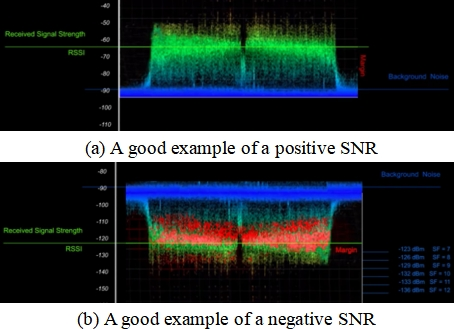
\includegraphics[width=0.6\linewidth]{fig2-3.png}
  \caption{example of a positive/negative SNR}
  \label{fig:2-3}
\end{figure}

\section{Existing Solutions}
\subsection{CFR-Based Physical Layer Key Generation}
One common approach to Physical layer key generation for LoRa is to use the fine-grained channel frequency response (CFR). Y. Peng et al. proposed a secret key generation method from CFR for OFDM TDD systems\cite{7054386}. Moreover, H. Luo et al. proposed a Channel Frequency Response-Based Secret Key Generation Scheme in In-Band Full-Duplex MIMO-OFDM Systems\cite{10158732}. When receiving \(I_{MS}\), both BS and MS construct a CFR estimate vector at the agreed subcarrier index set \(I_{MS}\) as
\begin{equation} 
  \hat{H}_{U}(I_{MS})   = \left [ \hat{H}_{U}(f_{(1)})\hat{H}_{U}(f_{(2)}) ...\hat{H}_{U}(f_{1(T_{b})}) \right ], where\ u\in \left \{ BS, MS  \right \}   
\end{equation} 
and then generate the secret key
\begin{equation} 
  K_{U}  = \left [ K_{U}({(1)})K_{U}{(2)} ...K_{U}({2T_{b}}) \right ]
\end{equation} 

The CFR is an unique characteristic of the LoRa channel that depends on the distance, orientation, and other environmental factors. By estimating the CFR at both ends of the communication link, the devices can generate a secret key that is shared only between them.
\subsection{RSSI-Based Physical Layer Key Generation}
Another approach to physical layer key generation for LoRa is to use the received signal strength indicator (RSSI). The RSSI is a measure of the strength of the received signal. S. Jana et al. evaluated the effectiveness of secret key extraction for private communication between two wireless devices from the received signal strength variations on the wireless channel between the two devices\cite{10.1145/1614320.1614356}. After that, W. Xu et al. employed a number of signal processing techniques to improve key generation rate significantly and proposed a novel compressive sensing-based reconciliation framework to reduce the mismatch rate\cite{8580375}. 
\begin{equation} y = y_{\mathrm{ Bob}}-y_{\mathrm{ Alice}}= A \left ({K_{\mathrm{ Bob}}-K_{\mathrm{ Alice}}}\right) + e= A x +e \end{equation} 
\begin{equation} \mathop {\mathrm {arg\,min}} _{x} \| x \|_{1} \quad \text {subject to}~ ~\left \|{y - Ax}\right \|_{2} < \epsilon.\end{equation} 
\begin{equation}K_{\mathrm{ Alice}}^{'} = K_{\mathrm{ Alice}} \oplus x\end{equation} 

The RSSI is also affected by the distance and other environmental factors. By exchanging RSSI measurements, the devices can generate a secret key that is shared only between them.

\subsection{Chaos-based Physical Layer Key Generation}
One another emerging technique for physical layer key generation in wireless networks is the use of chaos theory. The chaotic behavior of the wireless channel can be exploited to generate a random bit sequence that is used as a secret key shared only between the communicating devices. Yahya M. Al-Moliki et al. proposed a chaotic key creation approach, that is introduced by including the position-sensitive and real-valued channel state information of the VLC channel\cite{https://doi.org/10.1049/iet-opt.2018.5072}. 
\begin{equation}{\widehat {\mathbf{s}}_k} = \arg \mathop {\min }\limits_{{\mathbf{s}}_k^{(i)} \in {\mathbf{S}}} {\left\| {{{\mathbf{r}}^{(k)}} - {h_k}{\mathbf{s}}_k^{(i)}} \right\|^2};k = 1, \ldots ,K\end{equation}
where
\begin{equation}{{\mathbf{r}}^{(k)}} = \begin{cases} {\mathbf{r}}&{;{\text{ for }}k = 1} \\ {{{\mathbf{r}}^{(k - 1)}} - {h_{k - 1}}{{\widehat {\mathbf{s}}}_{k - 1}}}&{;{\text{ for }}k = 2, \ldots ,K.} \end{cases}\end{equation}
then, the output of the \(k^{th}\) stage is demodulated as \({{\hat{\mathbf b}}_k} = \left[ {\begin{array}{lll} {{{\hat b}_{k,1}}}& \ldots &{{{\hat b}_{k,U}}} \end{array}} \right]\).
The chaotic nature of the wireless channel ensures that the generated key is random and difficult to predict, making it difficult for adversaries to eavesdrop on the communication link.
\subsection{Deep-Learning-Based Physical Layer Key Generation}
A related approach to physical layer key generation for wireless network is the use of machine learning algorithms. Deep learning or machine learning algorithms can be used to analyze the wireless channel characteristics and identify patterns that can be used to generate a secret key. For example, by using supervised learning algorithms, the devices can analyze the wireless channel behavior and identify features that are unique to each communication link. These features can then be used to generate a unique secret key that is shared only between the devices. X. Zhang et al. implemented a Deep-Learning-Based Physical-Layer Secret Key Generation for FDD Systems using the adaptive moment estimation (ADAM) algorithm with the following loss function\cite{9526766}. 
\begin{equation} {\mathrm{ Loss}}_{\mathbb {D}}\left ({\boldsymbol {\Omega }}\right) = {\mathrm{ MSE}}\left ({\widehat {\mathbf {x}}_{2}, \mathbf {x}_{2}}\right)=\frac {1}{VN_{\mathbf {x}}}\sum _{v=0}^{V-1}\left \|{\widehat {\mathbf {x}}_{2}^{\left ({v}\right)} -\mathbf {x}_{2}^{\left ({v}\right)}}\right \|_{2}^{2}\end{equation} 
\subsection{Quantum-Based Physical Layer Key Distribution}
Using quantum mechanics principles for physical layer key distribution is also a promising approach for wireless networks. Quantum mechanics principles can be applied to generate truly random keys using the quantum states of particles. The devices can use quantum states of particles to generate random bits that are used as secret keys for encrypting and decrypting their communication. Using quantum keys ensures that the key is truly random and cannot be predicted or intercepted by an adversary. However, several technical limitations, such as channel losses and transmission distance, should be overcome before it comes to practical application.

\section{Advantages and Disadvantages}
Firstly, chaos theory for physical layer key generation in wireless networks has several strengths and weaknesses. On the one hand, the chaotic behavior of the wireless channel ensures that the generated key is random and difficult to predict, making it difficult for adversaries to eavesdrop on the communication link. This approach provides high security and randomness, which is essential for secure communication. However, on the other hand, using chaos theory for physical layer key generation may be challenging in practical implementation. The chaotic behavior of the wireless channel may be difficult to characterize and control in practical environments, making it difficult to ensure consistent and reliable key generation. Also, chaos theory may be more complex mathematical than other key generation techniques, making it challenging to implement and scale in resource-constrained environments.

Secondly, using quantum-based principles for physical layer key distribution in wireless networks has several strengths and weaknesses. On the one hand, quantum keys ensure that the key is truly random and cannot be predicted or intercepted by an adversary, providing high security and randomness. This approach is auspicious for ensuring secure communication in wireless networks. However, on the other hand, the quantum-based is typically designed for optical fiber or free-space optical communication, not for RF wireless communication like LoRa. The use of quantum mechanics principles may be challenging in practical implementation. Generating quantum keys requires using specialized quantum devices and technologies that may not be widely available or practical for resource-constrained environments. Additionally, quantum communication is weaker to practical imperfections than classical communication, making it difficult to ensure consistent and reliable key distribution under practical conditions. 

Thirdly, the Deep-learning-based method offers promising security and key establishment advantages without pre-shared secrets. However, it also faces challenges related to data quality, model vulnerabilities, and resource constraints. It is not a standard or suitable choice for LoRa technology due to resource constraints, data availability, real-time requirements, complexity, and the presence of established security measures within the LoR protocol. Implementing Deep-Learning-Based LoRa networks would require overcoming these challenges and aligning with the specific requirements and limitations of LoRa technology.

Such three methods fundamentally differ in operating principles, resource requirements, environmental sensitivity, standardization, and security considerations. Typically, the hardware performance of LoRa nodes, including the CPU and memory specifications limitation, is designed for Low-Power and Battery-Operated, which means they are not providing such calculation performance.

Thus, no matter in theory or industrial area, most research on the Physical-Layer Secret Key Generation for LoRa are based on their wireless channel characteristics as very fast and efficient to implement in LoRa Node.

\section{Relationship with Proposed Solution}
In the context of the guide study, the primary focus revolves around the inherent characteristics of the Internet of Things. Given the inherent constraints imposed by the limited computational capacity of LoRa nodes and a spectrum of attributes, including communication speed and error rates, I have elected to adopt a widely acknowledged approach within the industry. This approach, rooted in the Received Signal Strength Indicator principles, serves as the foundation for the generation of physical-layer cryptographic keys. Moreover, my methodology draws inspiration from established practices documented in pertinent literature. To enhance the quality of the raw signal data, I intend to implement a series of preprocessing techniques, encompassing bit quantization and signal demodulation.

The present study and research direction exhibit significant potential, particularly within the realm of the Internet of Things and the nuanced field of physical-layer key generation facilitated by LoRa technology. 

Preprocessing Methodologies: In the context of managing RSSI data, the employment of advanced preprocessing techniques assumes paramount importance. Strategies such as bit quantization and signal demodulation should be explored in depth, and their application should be calibrated to optimize precision and accuracy.

An inclusive and thorough approach to validation should be adopted, spanning a spectrum of operational contexts that encapsulate the diversity of real-world IoT deployment scenarios. Rigorous validation across an array of settings, encompassing both indoor and outdoor environments, as well as scenarios with varying degrees of obstruction, will ensure the adaptability and efficacy of the proposed method.

Furthermore, I have meticulously devised a comprehensive validation strategy tailored to the real-world deployment scenarios characteristic of LoRa technology. The testing plan includes but is not limited to the potential critical use case for LoRa technology, which is in the field of environmental monitoring. By doing so, I endeavor to substantiate the practical applicability of the theoretical framework I have laid out. Also, the methodical planning and meticulous experimental design are the cornerstones of empirical validation. The experimental framework should be meticulously devised to yield a substantial corpus of empirical evidence, reflecting the manifold operational contexts under scrutiny.
